% Options for packages loaded elsewhere
\PassOptionsToPackage{unicode}{hyperref}
\PassOptionsToPackage{hyphens}{url}
%
\documentclass[
]{article}
\usepackage[colorlinks = true,
linkcolor = blue,
urlcolor  = blue,
citecolor = blue,
anchorcolor = blue]{hyperref}
\usepackage{lmodern}
\usepackage{amssymb,amsmath}
\usepackage{ifxetex,ifluatex}
\usepackage{subcaption}
\usepackage{float}
\captionsetup{compatibility=false}
\ifnum 0\ifxetex 1\fi\ifluatex 1\fi=0 % if pdftex
  \usepackage[T1]{fontenc}
  \usepackage[utf8]{inputenc}
  \usepackage{textcomp} % provide euro and other symbols
\else % if luatex or xetex
  \usepackage{unicode-math}
  \defaultfontfeatures{Scale=MatchLowercase}
  \defaultfontfeatures[\rmfamily]{Ligatures=TeX,Scale=1}
\fi
% Use upquote if available, for straight quotes in verbatim environments
\IfFileExists{upquote.sty}{\usepackage{upquote}}{}
\IfFileExists{microtype.sty}{% use microtype if available
  \usepackage[]{microtype}
  \UseMicrotypeSet[protrusion]{basicmath} % disable protrusion for tt fonts
}{}
\makeatletter
\@ifundefined{KOMAClassName}{% if non-KOMA class
  \IfFileExists{parskip.sty}{%
    \usepackage{parskip}
  }{% else
    \setlength{\parindent}{0pt}
    \setlength{\parskip}{6pt plus 2pt minus 1pt}}
}{% if KOMA class
  \KOMAoptions{parskip=half}}
\makeatother
\usepackage{xcolor}
\IfFileExists{xurl.sty}{\usepackage{xurl}}{} % add URL line breaks if available
\IfFileExists{bookmark.sty}{\usepackage{bookmark}}{\usepackage{hyperref}}
\hypersetup{
  hidelinks,
  pdfcreator={LaTeX via pandoc}}
\urlstyle{same} % disable monospaced font for URLs
\usepackage{longtable,booktabs}
% Correct order of tables after \paragraph or \subparagraph
\usepackage{etoolbox}
\makeatletter
\patchcmd\longtable{\par}{\if@noskipsec\mbox{}\fi\par}{}{}
\makeatother
% Allow footnotes in longtable head/foot
\IfFileExists{footnotehyper.sty}{\usepackage{footnotehyper}}{\usepackage{footnote}}
\makesavenoteenv{longtable}
\usepackage{graphicx}
\makeatletter
\def\maxwidth{\ifdim\Gin@nat@width>\linewidth\linewidth\else\Gin@nat@width\fi}
\def\maxheight{\ifdim\Gin@nat@height>\textheight\textheight\else\Gin@nat@height\fi}
\makeatother
% Scale images if necessary, so that they will not overflow the page
% margins by default, and it is still possible to overwrite the defaults
% using explicit options in \includegraphics[width, height, ...]{}
\setkeys{Gin}{width=\maxwidth,height=\maxheight,keepaspectratio}
% Set default figure placement to htbp
\makeatletter
\def\fps@figure{htbp}
\makeatother
\setlength{\emergencystretch}{3em} % prevent overfull lines
\providecommand{\tightlist}{%
  \setlength{\itemsep}{0pt}\setlength{\parskip}{0pt}}
\setcounter{secnumdepth}{-\maxdimen} % remove section numbering
\ifluatex
  \usepackage{selnolig}  % disable illegal ligatures
\fi

\author{}
\date{}
\newcommand{\hhref}[3][blue]{\href{#2}{\color{#1}{#3}}}%
\begin{document}

\begin{titlepage}
	\begin{center}
		\vspace*{1cm}
		
		\textbf{Automatic splitting into scenes of gameplay videos}
		
		\vspace{0.5cm}
		\hhref{https://github.com/diegoami/DA_ML_Capstone}{https://github.com/diegoami/DA\_ML\_Capstone}
		
		\vspace{1.5cm}
		
		\textbf{Diego Amicabile}
		
		\vfill
		
		Final Capstone Project for the Machine Learning Engineering Nanodegree
		\vspace{0.8cm}
	
		\textbf{Udacityb}
		
		\vspace{0.8cm}
		

		2 November 2020
		
	\end{center}
\end{titlepage}

\hypertarget{definition}{%
\section{DEFINITION}\label{definition}}

\hypertarget{project-overview}{%
\subsection{PROJECT OVERVIEW}\label{project-overview}}

During the last few years it has become more and more common to stream
on platforms such as Youtube and Twitch while playing video games, or to
upload recorded sessions. The volume of videos produced is overwhelming.
In many of the video games being streamed there are different types of
scenes. Both for content producers and consumers it would be useful to
be able to automatically split videos, to find out in what time
intervals different types of scenes run. 

The game that I have chosen to analyze is \emph{Mount of Blade:
Warband}, of which I attempted several walkthroughs. In this game, you command a hero, and later on a warband,  in their quest to power in the fictitious continent of Calradia, divided between six warring factions. On their way there you have to fight battles, sieges, tournaments, clear bandit handouts, fulfill quests in what is usually a very long game, spanning hundreds of hours.

You spend most of the time on a ``strategic map'', taking your warband to
any of the towns or villages, following or running away from other
warbands which can belong to friendly or rival factions, or looking for
quest objectives.


\begin{figure}[H]
	\centering
	\begin{subfigure}[b]{0.3\textwidth}
		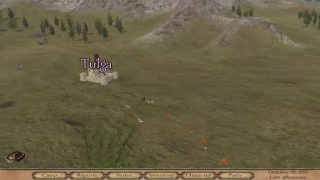
\includegraphics[width=\linewidth]{docimages/E_0041_00_09_28.jpg}
		\caption{Close to a town}
	\end{subfigure}
	\begin{subfigure}[b]{0.3\textwidth}
		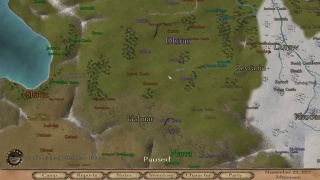
\includegraphics[width=\linewidth]{docimages/E_0049_00_15_38.jpg}
		\caption{Bird's view}
	\end{subfigure}
	\begin{subfigure}[b]{0.3\textwidth}
		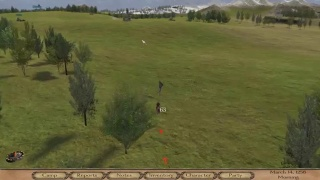
\includegraphics[width=\linewidth]{docimages/E_0063_00_17_06.jpg}
		\caption{Your warband}
	\end{subfigure}
\end{figure}


Other in-game screenshots can show the character's inventory, warband
composition, allow interaction with non-playing characters (NPCs), display status
messages\ldots{}


\begin{figure}[H]
	\centering
	\begin{subfigure}[b]{0.3\textwidth}
		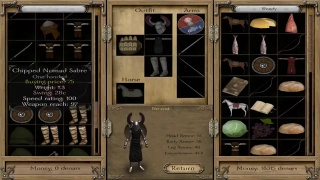
\includegraphics[width=\linewidth]{docimages/E_0056_00_31_30.jpg}
		\caption{In a shop}
	\end{subfigure}
	\begin{subfigure}[b]{0.3\textwidth}
		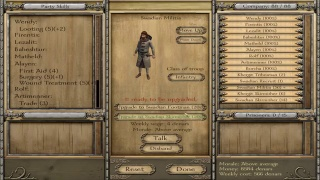
\includegraphics[width=\linewidth]{docimages/E_0056_00_58_08.jpg}
		\caption{Manage your warband}
	\end{subfigure}
	\begin{subfigure}[b]{0.3\textwidth}
		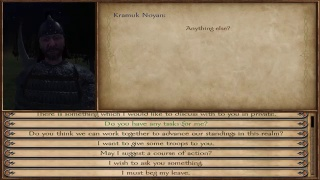
\includegraphics[width=\linewidth]{docimages/E_0059_00_26_26.jpg}
		\caption{Talk to a NPC}
	\end{subfigure}
\end{figure}


The hero can also take a walk in town, villages and castles, have training sessions with soldiers, or spar with them in arena.


\begin{figure}[H]
	\centering
	\begin{subfigure}[b]{0.3\textwidth}
		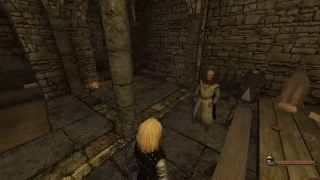
\includegraphics[width=\linewidth]{docimages/E_0055_00_33_54.jpg}
		\caption{In a noble's castle}
	\end{subfigure}
	\begin{subfigure}[b]{0.3\textwidth}
		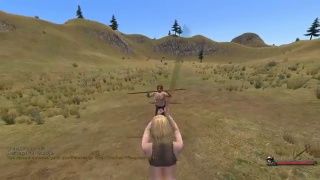
\includegraphics[width=\linewidth]{docimages/E_0064_00_52_16.jpg}
		\caption{Training Session}
	\end{subfigure}
	\begin{subfigure}[b]{0.3\textwidth}
		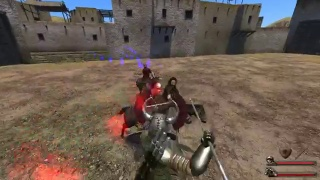
\includegraphics[width=\linewidth]{docimages/E_0076_00_42_48.jpg}
		\caption{Challenge in the arena}
	\end{subfigure}
\end{figure}

However, what we are interested in is locating the scenes when the
warband engages enemies and the game switches to a tactical view, such
as a battle in an open field or in a village\ldots{}

\begin{figure}[H]
	\centering
	\begin{subfigure}[b]{0.3\textwidth}
		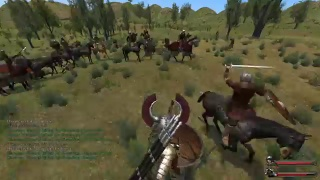
\includegraphics[width=\linewidth]{docimages/E_0060_00_44_20.jpg}
		\caption{Raid on caravan}
	\end{subfigure}
	\begin{subfigure}[b]{0.3\textwidth}
		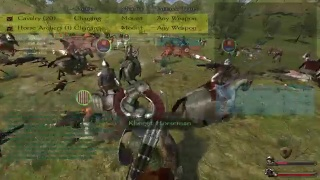
\includegraphics[width=\linewidth]{docimages/E_0066_01_21_18.jpg}
		\caption{Major battle}
	\end{subfigure}
	\begin{subfigure}[b]{0.3\textwidth}
		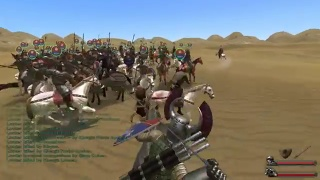
\includegraphics[width=\linewidth]{docimages/E_0065_00_29_08.jpg}
		\caption{Desert battle}
	\end{subfigure}
\end{figure}

or when they siege a town or a castle...

\begin{figure}[H]
	\centering
	\begin{subfigure}[b]{0.3\textwidth}
		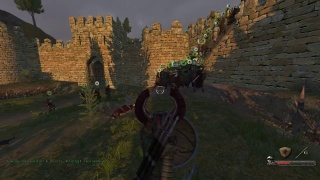
\includegraphics[width=\linewidth]{docimages/E_0068_00_48_04.jpg}
		\caption{Unuzdaq castle}
	\end{subfigure}
	\begin{subfigure}[b]{0.3\textwidth}
		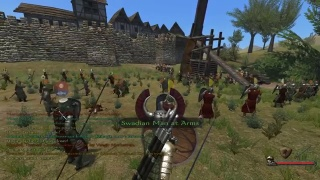
\includegraphics[width=\linewidth]{docimages/E_0068_00_20_08.jpg}
		\caption{Dhirim}
	\end{subfigure}
	\begin{subfigure}[b]{0.3\textwidth}
		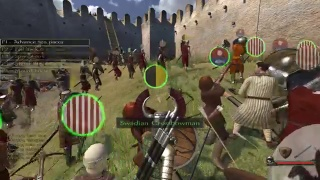
\includegraphics[width=\linewidth]{docimages/E_0075_00_25_50.jpg}
		\caption{Halmar}
	\end{subfigure}
\end{figure}

or when they assault a bandit hideout.



\begin{figure}[H]
	\centering
	\begin{subfigure}[b]{0.3\textwidth}
		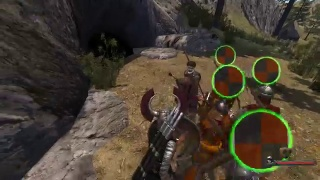
\includegraphics[width=\linewidth]{docimages/E_0041_00_39_58.jpg}
		\caption{Forest bandits}
	\end{subfigure}
	\begin{subfigure}[b]{0.3\textwidth}
		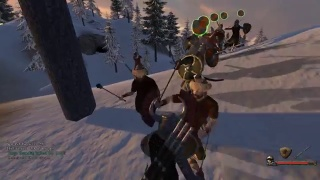
\includegraphics[width=\linewidth]{docimages/E_0054_00_10_54.jpg}
		\caption{Tundra bandits}
	\end{subfigure}
	\begin{subfigure}[b]{0.3\textwidth}
		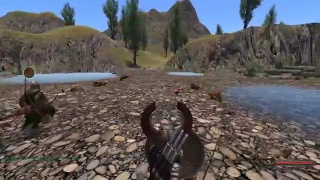
\includegraphics[width=\linewidth]{docimages/E_0042_00_05_08.jpg}
		\caption{Steppe bandits}
	\end{subfigure}
\end{figure}



The hero often takes part in tournaments, which are a very important
part of the gam, and which we want to locate in gameplay videos. Regrettably, they may look similar to situations like training or sparring in the arena, that are not very interesting.



\begin{figure}[H]
	\centering
	\begin{subfigure}[b]{0.3\textwidth}
		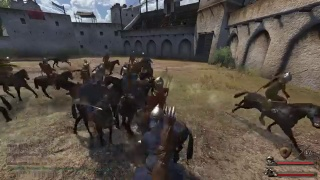
\includegraphics[width=\linewidth]{docimages/E_0057_00_21_48.jpg}
		\caption{Tulga tournament}
	\end{subfigure}
	\begin{subfigure}[b]{0.3\textwidth}
		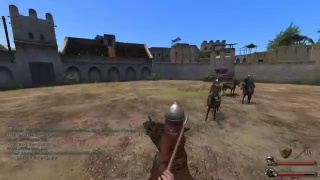
\includegraphics[width=\linewidth]{docimages/E_0061_00_25_56.jpg}
		\caption{Tulga tournament}
	\end{subfigure}
	\begin{subfigure}[b]{0.3\textwidth}
		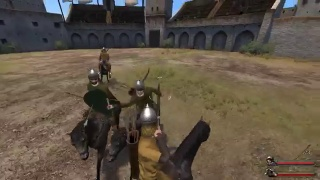
\includegraphics[width=\linewidth]{docimages/E_0042_00_12_48.jpg}
		\caption{Tulga tournament}
	\end{subfigure}
\end{figure}


Quests and ambushes, are pretty infrequent and the screenshots may look
similar to those of more peaceful situations. For instance when the hero is rescuing a lord from prison, or fighting a bandit in a village, are not very different from scenes when he might be just taking a stroll in a town or village.


\begin{figure}[H]
	\centering
	\begin{subfigure}[b]{0.3\textwidth}
		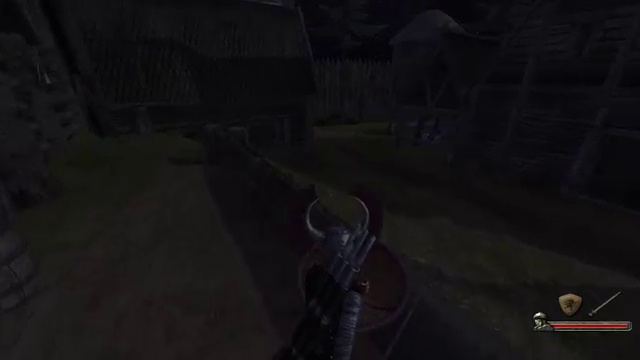
\includegraphics[width=\linewidth]{docimages/E_0054_00_40_24.jpg}
		\caption{Lord Rescue}
	\end{subfigure}
	\begin{subfigure}[b]{0.3\textwidth}
		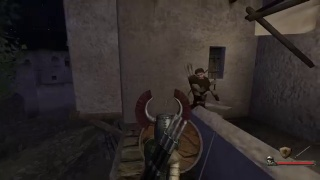
\includegraphics[width=\linewidth]{docimages/E_0063_00_27_08.jpg}
		\caption{Ambush in Town}
	\end{subfigure}
	\begin{subfigure}[b]{0.3\textwidth}
		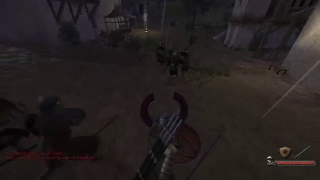
\includegraphics[width=\linewidth]{docimages/E_0067_00_52_32.jpg}
		\caption{Ambush in village}
	\end{subfigure}
\end{figure}


\newpage


\hypertarget{problem-statement}{%
\subsection{PROBLEM STATEMENT}\label{problem-statement}}

The goal is to create and deploy a model which is able to classify
images from the game \emph{Mount\&Blade: Warband} and return a category,
such as ``Battle'', ``Hideout'', ``Siege'', ``Tournament'' and
``Other'' for each frame.

The approach should be robust enough to allow for later expanding of categories, for which there are not enough samples at the moment.
It would be ideal to have categories for less frequent scenes such as "Prison escape", "Ambush", "Quest", but this will be out of scope and such scenes will be lumped together with the closest category).

An additional goal is to have a model which identifies contiguous scenes in a gameplay video of \emph{Mount\&Blade: Warband}, providing the beginning and the end of the scenes, and their most likely categories.

A necessary requirement for this project is to gather a dataset of screenshots from gameplay videos, as well as the category to which they belong.

\hypertarget{metrics}{%
\subsection{METRICS}\label{metrics}}

While training, validating and testing the image classifier model, I will evaluate it  by means of accuracy and cross-entropy loss.
While overall accuracy is not a good metrics in an unbalanced dataset, cross-entropy loss is a good loss function for Classification Problems with several classes, as it minimizes the distance between the predicted and the actual probability.

I will also use scikit-learn functions to measure precision, recall, accuracy and F1, for each class and on average, as well as to calculate a total weighted and mean accuracy. A model will not be considered good enough if it cannot deliver a good precision and, even more importantly, recall on classes that have relatively few samples.

\hypertarget{analysis}{%
\section{ANALYSIS}\label{analysis}}

Most files referenced in these section are relative to \hhref{https://github.com/diegoami/DA_ML_Capstone/}{this Github repository}..


\hypertarget{data-exploration}{%
\subsection{DATA EXPLORATION}\label{data-exploration}}

\hypertarget{creating-a-dataset}{%
\subsubsection{CREATING A DATASET}\label{creating-a-dataset}}

To create a dataset I took some videos from a game walkthrough of mine,
the adventures of Wendy (\hhref{https://www.youtube.com/playlist?list=PLNP_nRm4k4jfNLo7FkjXewFH9Xe5Uc2Pa}{I}, \hhref{https://www.youtube.com/playlist?list=PLNP_nRm4k4jd-AJ0GwTPS1ld2YP8FdT4h}{II}). 
I used the episodes from 41 to 68 to build the model, keeping episodes 69 to 77 to test it, and to simplify download I also created following playlists on youtube, containing just the episodes I will be using in this project:

\begin{itemize}
\tightlist
\item
  \hhref{https://www.youtube.com/playlist?list=PLNP_nRm4k4jfVfQobYTRQAXV\_uOzt8Bov}{CNN-Wendy-I}
\item
  \hhref{https://www.youtube.com/playlist?list=PLNP_nRm4k4jdEQ-OM31xNqeE64svvx-aT}{CNN-Wendy-II}
\item
  \hhref{https://www.youtube.com/playlist?list=PLNP_nRm4k4jeoJ8H7mtTUbbOJ6_Rx_god}{CNN-Wendy-III}
\end{itemize}

To build a dataset, I identified scenes in these episodes and wrote them all down in the video description on youtube. 

For instance, in episode 54, I have wrote down following scenes in the description, of the
category ``Hideout'', ``Battle'', ``Tournament'', ``Town'' (``Town'' is
eventually remapped to ``Battle'') - first word of the description line. All the other parts of the video are
categorized as ``Other''.   

\begin{itemize}
\tightlist
\item
  09:51-12:21 Hideout Tundra Bandits (Failed)
\item
  18:47-19:44 Battle with Sea Raiders
\item
  20:50-21:46 Battle with Sea Raiders
\item
  22:54-23:42 Battle with Sea Raiders
\item
  34:06-37:44 Tournament won in Tihr
\item
  38:46-40:48 Town escape for Boyar Vlan
\end{itemize}

\hypertarget{companion-projects}{%
\subsubsection{COMPANION PROJECT}\label{companion-projects}}

To prepare the data set, I created \hhref{https://github.com/diegoami/DA_split_youtube_frames\_s3/}{a companion project} allowing to:

\begin{itemize}
\tightlist
\item
  download the relevant videos from youtube, using the
  \emph{youtube-dl} python library, in a 640x360 format
\item
  extract at every two seconds a frame and save it in \emph{jpeg} file, using
  the \emph{opencv} python library, resizing to the practical format
  320x180
\item
  download the text from the youtube descriptions, which describes the scenes, and save it along the
  video as \emph{metadata}
\item
  assign the images created in the second step to labels, according to the metadata produced at step 3
\item 
  save images into subdirectories named after the labels they ere assigned   
\end{itemize}


The result of this process has been uploaded \hhref{https://da-youtube-ml.s3.eu-central-1.amazonaws.com/}{to a public bucket on Amazon S3}, from where you can browse and download all files produced in the above described stages.

\hypertarget{dataset-characteristics}{%
\subsubsection{DATASET CHARACTERISTICS}\label{dataset-characteristics}}

The dataset contains 51216 images, 320 x 180, in jpeg format,
distributed over the following classes. It can be downloaded and extracted from \hhref{https://da-youtube-ml.s3.eu-central-1.amazonaws.com/wendy-cnn/frames/wendy_cnn_frames_data_5.zip}{this zip file on S3}.

\begin{longtable}[]{@{}llll@{}}
\toprule
& Category & Amount & Percentage\tabularnewline
\midrule
\endhead
& Battle & 7198 & 14.0\%\tabularnewline
& Hideout & 1163 & 2.2\%\tabularnewline
& Other & 35425 & 67.4\%\tabularnewline
& Siege & 634 & 1.2\%\tabularnewline
& Tournament & 6796 & 13.3\%\tabularnewline
& TOTAL & 51216 &\tabularnewline
\bottomrule
\end{longtable}

You can browse them using the \emph{analysis.ipynb} notebooks. While
having a look at images, it seemed to me that a format of 320x180, in
grayscale, keeps most of the information necessary to categorize it. 

\hypertarget{exploratory-visualization}{%
\subsubsection{EXPLORATORY
VISUALIZATION}\label{exploratory-visualization}}

Using PCA on a flattened version of the image matrixes, in format 80x45,
black and white, I produced visualizations of the distribution of the 2 main principal components of the full dataset. 

\begin{figure}[H]
\centering
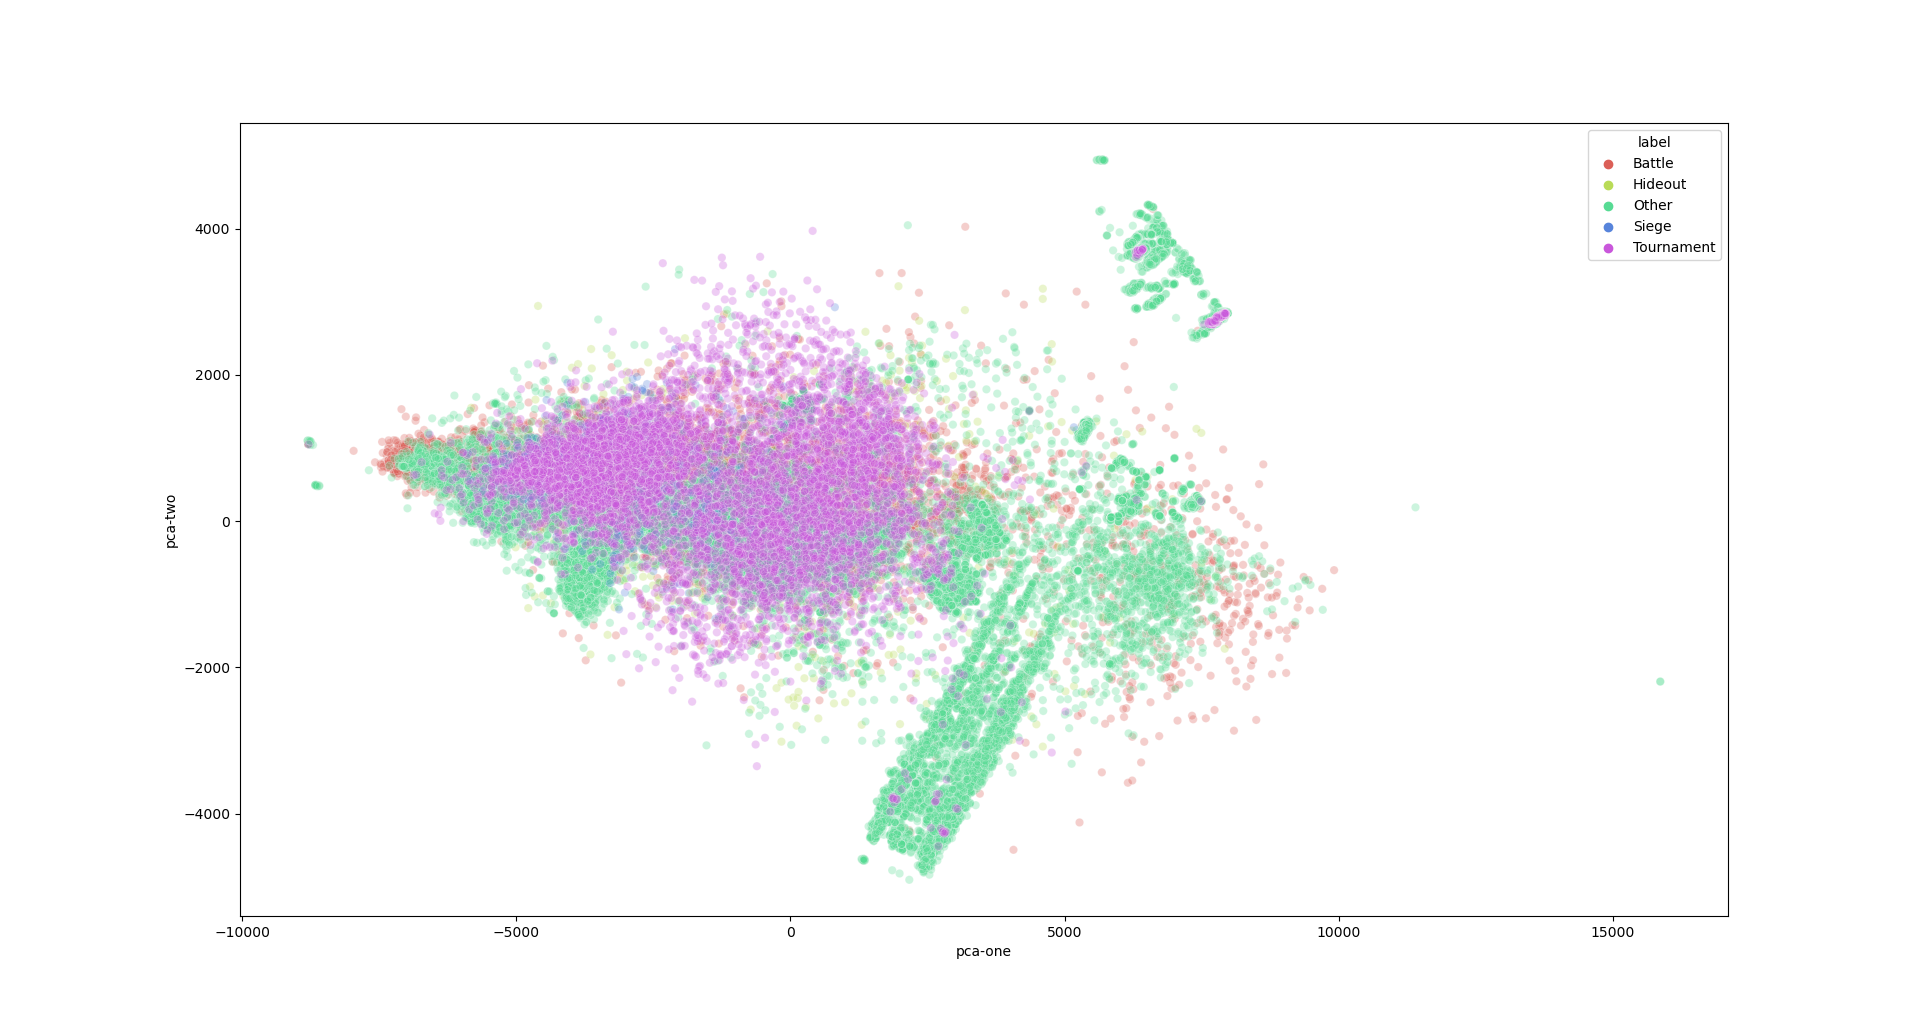
\includegraphics{visualizations/pca_sklearn_2d_80_45_L.png}
\caption{2 Main Principal Components}
\end{figure}

and also of the three main principal components, using the same color scheme.

\begin{figure}[H]
	\centering
	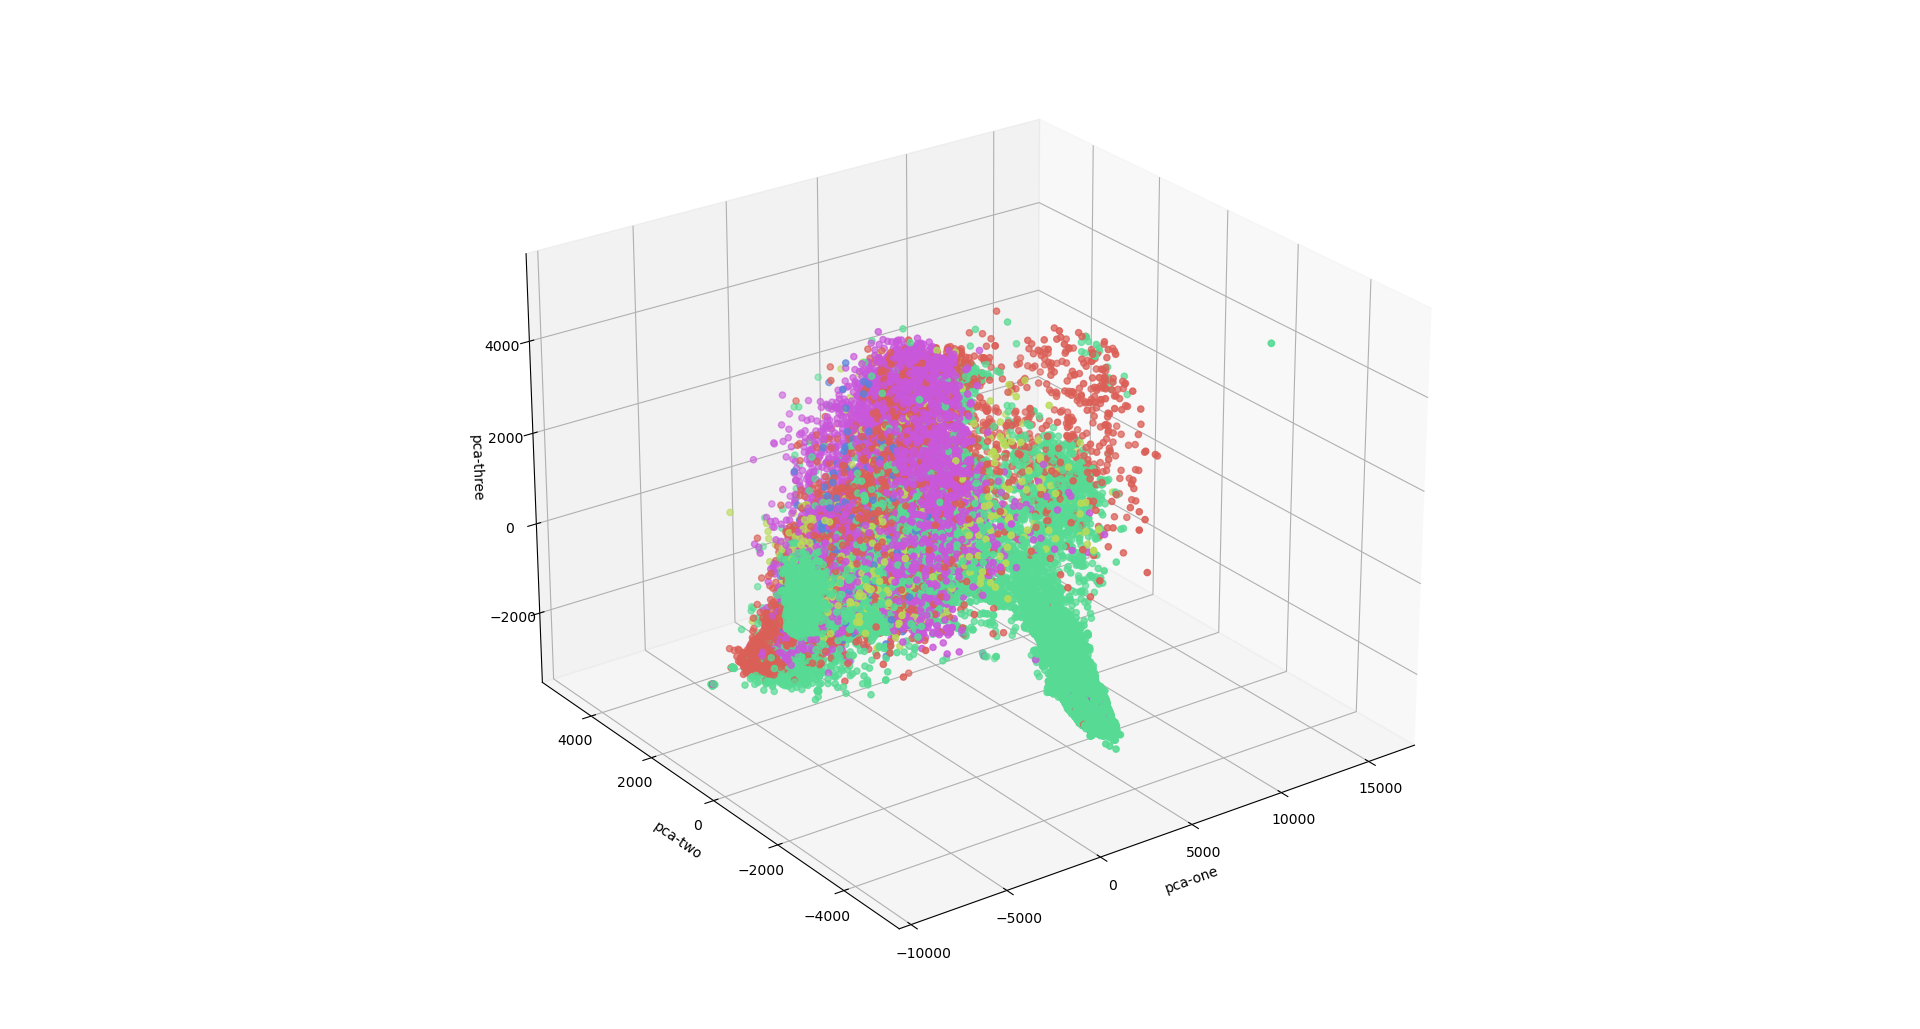
\includegraphics{visualizations/pca_sklearn_3d_80_45_L.png}
	\caption{3 Main Principal Components}
\end{figure}


It can be seen that ``Other'' scenes are separated in several clusters.
``Battle'', ``Tournament'', ``Siege'' and ``Hideout'' images do group in
certain regions, but there is a lot of overlap between themselves and
with some of the ``Other'' images.

Later on, after we have create a VGG13 model, we can plot an alternative PCA representation of the
dataset, using the additional generated features that can be recovered from the last layer of the neural net.

\begin{figure}[H]
\centering
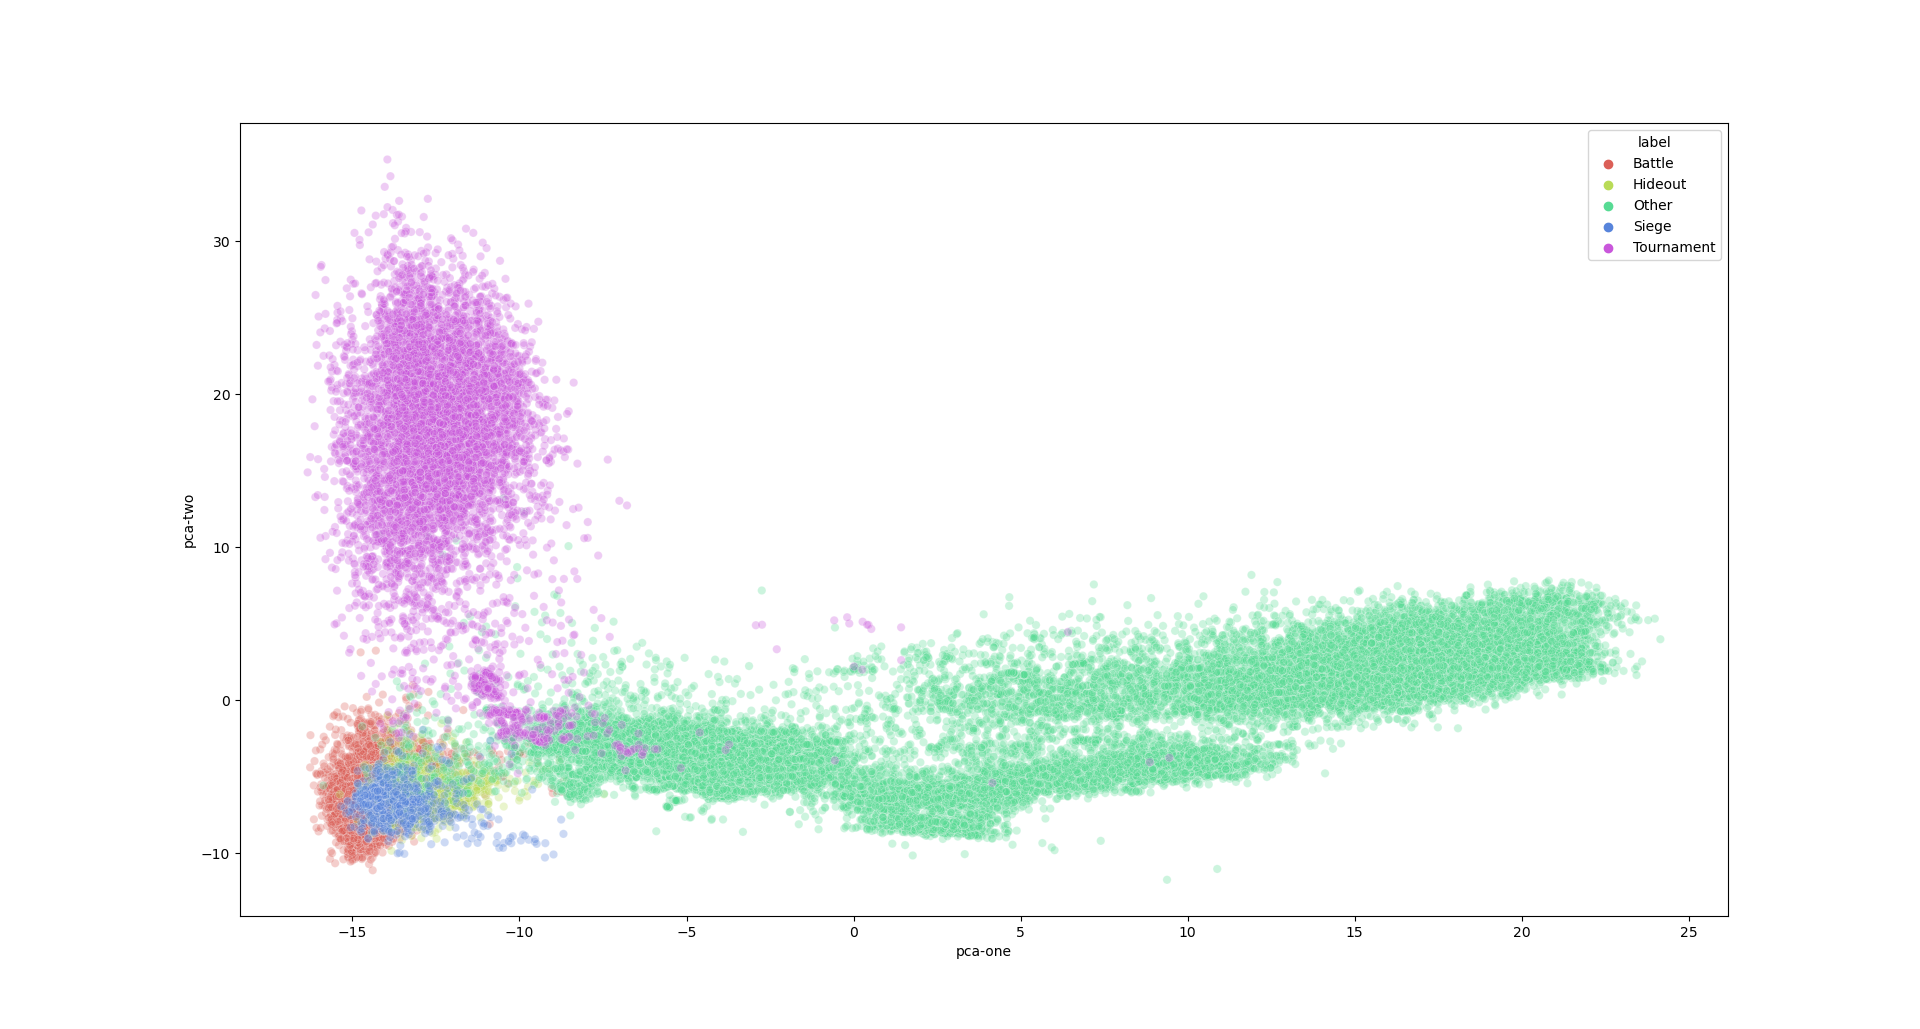
\includegraphics{visualizations/pca_v5n_2d_f.png}
\caption{VGG13-2 principal components}
\end{figure}

\begin{figure}[H]
\centering
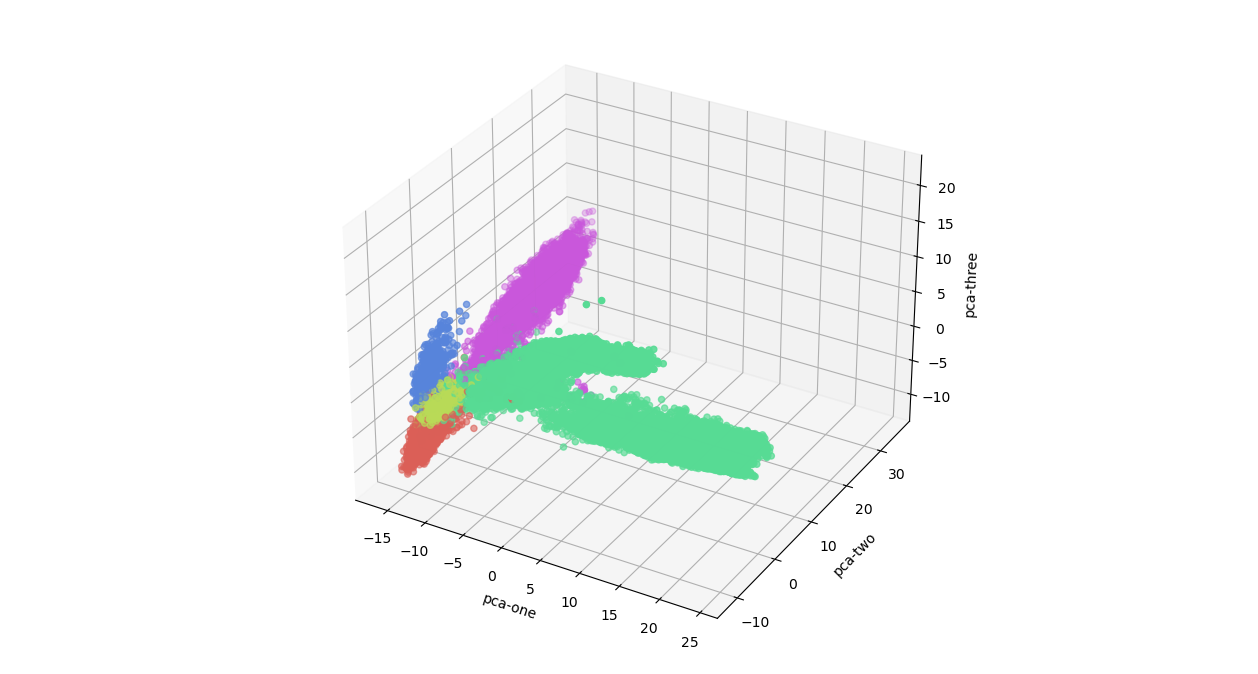
\includegraphics{visualizations/pca_v5n_3d_f4.png}
\caption{VGG13-3 principal components}
\end{figure}

Here there are is much less overlap between regions where the different
classes are located. That shows how the features created in a neural network are
important for the categorization task.

The script used to produce these visualzations are \emph{pca\_vgg.py} and \emph{pca\_sklearn.py}  

\hypertarget{algorithms-and-techniques}{%
\subsection{ALGORITHMS AND
TECHNIQUES}\label{algorithms-and-techniques}}

The general idea is to create first an image classifier to categorize the
images extracted from gameplay videos. Then to use the predictions generated by the image classifier as a base for splitting gameplay videos into scenes.

The main approach to build an Image Classifier will be  Convolutional
Neural Network, since

\begin{itemize}
\tightlist
\item
  this is a well-tried way to approach the problem
\item
  I can use standard CNN topologies available in Pytorch, such as VGG,
  picking one with the best tradeoff performance/complexity
\item
  at the very least the model would give me more information on
  what I have to be looking for
\end{itemize}

A simple to use and flexible topology I decided to use was VGG13, which is
powerful enough to give good results and small enough to fit on the GPU I used for training.

As the images extracted from game walkthroughs are not related to real
world images, using a pre-trained net and expanding it with transfer
learning did not seem a sensible approach. Instead, I opted for a full
train.

\hypertarget{benchmark}{%
\subsection{BENCHMARK}\label{benchmark}}

As 67.4 \% of the images belong to the category ``Other'', a model
should have an accuracy of at least 68\% for being considered better
than a model that always picks the Category ``Other''.

On top of that, I created a very simple model that uses flattened
matrixes of images as an input to standard scikit-learn
transformers and PCA.

Using greyscale images in 80x45 format, I got the following results
using Random Tree Forest and Stochastic Gradient Descent on 100 PCA-produced features, from a
validation set (which had not been used for training).

It is not surprising that these results do not look that bad at all, and
are actually good as separating ``Other'' images from images depicting
any kind of engagement / fight (Tournament, Battle, Siege, Hideout).
That is expected, as there are some GUI components that appear only in
these scenes.

\hypertarget{randomforestclassifier}{%
\paragraph{RandomForestClassifier}\label{randomforestclassifier}}

\begin{verbatim}
RandomForestClassifier(n_estimators=200)
Accuracy: 0.932
F1 Score: 0.926

              precision    recall  f1-score   support

           0       0.83      0.91      0.87      2375
           1       0.99      0.18      0.31       384
           2       0.98      0.97      0.98     11691
           3       1.00      0.34      0.51       209
           4       0.81      0.92      0.86      2243

    accuracy                           0.93     16902
   macro avg       0.92      0.67      0.70     16902
weighted avg       0.94      0.93      0.93     16902
\end{verbatim}


\hypertarget{sgdclassifier}{%
\paragraph{SGDClassifier}\label{sgdclassifier}}

\begin{verbatim}
SGDClassifier(alpha=0.001, max_iter=10000)
Accuracy: 0.841
F1 Score: 0.843

              precision    recall  f1-score   support

           0       0.72      0.53      0.61      2375
           1       0.53      0.37      0.44       384
           2       0.97      0.93      0.95     11691
           3       0.56      0.30      0.39       209
           4       0.52      0.83      0.64      2243

    accuracy                           0.84     16902
   macro avg       0.66      0.59      0.60     16902
weighted avg       0.86      0.84      0.84     16902
\end{verbatim}


\hypertarget{methodology}{%
\section{METHODOLOGY}\label{methodology}}

\hypertarget{data-processing}{%
\subsection{DATA PROCESSING}\label{data-processing}}

The image dataset has been created extracting frames from videos on
youtube, and putting them in subdirectories named like the category they
belong with. 

These images have also been resized are in 320 x 180, RGB format, and
normalized.

While training the benchmark models, images are transformed into
grayscale and resized to 80 x 45, but when training the deep learning
models we use the original images without resizing them, 320x180, and in color. 
This is because this is what the VGG models expect.

As these images originate from video games, any kind of data
augmentation such as mirrored or cropped images do not make sense. These artificially produced 
images would not be produced by the videogame, as for instance many GUI components are
always on the same side of the screen.

\hypertarget{implementation}{%
\subsection{IMPLEMENTATION}\label{implementation}}

I created scripts and notebooks so that they would work both locally and
on Sagemaker. For more details see the file \url{README.md} in the \hhref{https://github.com/diegoami/DA_ML_Capstone}{Github repository}

\hypertarget{training-script}{%
\paragraph{TRAINING SCRIPT}\label{training-script}}

The training script \emph{train.py}:

\begin{itemize}
\tightlist
\item
  uses an image loader from pytorch to create a generator scanning all
  files in the data directory.
\item
  uses a pytorchvision transformer to resize and normalize images
\item
  splits the dataset in train, validation and test sets, using
  stratification and shuffling
\item
  loads a VGG13 neural network, modified so that the output layers produce
  a category from our domain (5 categories in the final version)
\item
  For each epoch, execute a training step and evaluation step, trying to
  minimize the cross entropy loss in the validation set
\item
  Save the model so that it can be further used by the following steps
\item
  Evaluate the produced model on the test dataset, and print a
  classification report and a confusion matrix.
\end{itemize}

\hypertarget{verification-script}{%
\paragraph{VERIFICATION SCRIPT}\label{verification-script}}

The verification script \emph{verify\_model.py} works only locally, as
it assumes the model and the dataset has been saved locally from the previous
step. This script

\begin{itemize}
\tightlist
\item
  Loads the model created in the previous step
\item
  Walks through all the images in the dataset, one by one, returning a list a predictions (by means of the predictor)  and a list of truth values
\item
  prints average accuracy, a classification report based on
  discrepancies, a confusion matrix, and a list of images whose
  predicted category does not coincide with their labels, so that the
  dataset can be corrected.
\end{itemize}

\hypertarget{predictor}{%
\paragraph{PREDICTOR}\label{predictor}}

The file \emph{predict.py} contains the methods that are necessary to
deploy the model to an endpoint. It works both locally and on a
Sagemaker container and requires a previously trained model.

\begin{itemize}
\tightlist
\item
  input\_fn: this is be the endpoint entry point, which converts a Numpy
  matrix payload to a Pillow Image, applying the same preprocessing
  steps as during training
\item
  model\_fn: predicts a category using a previously trained model,
  accepting an image from the domain space (a screenshot from
  \emph{Mount\&Blade: Warband} in format 320 x 180) and transformed in
  the same way as during training
\item
  output\_fn: returns the model output as a numpy array: a list of log
  probabilites for each class
\end{itemize}

\hypertarget{endpoint}{%
\paragraph{ENDPOINT}\label{endpoint}}

The file \emph{endpoint.py} contains a method \emph{evaluate} allowing
to call an endpoint on Sagemaker, so that you can collect predictions,
which can be used to show a classification report and a confusion
matrix. It requires locally saved data, but the model is accessed
through a published endpoint, unlike the \emph{verify\_model.py}
component which requires a saved model locally.

\emph{endpoint.py} works only in Sagemaker, when called from a Jupyter
Notebook. An examples can be found in
\emph{CNN\_Fourth\_iteration.ipynb}.


\hypertarget{refinement}{%
\subsection{REFINEMENT}\label{refinement}}

How the approach evolved can be seen in the Jupyter Notebooks:  \emph{CNN\_First\_Iteration.ipynb}, \emph{CNN\_Second\_Iteration.ipynb},  \emph{CNN\_Third\_Iteration.ipynb} and \emph{CNN\_Fourth\_Iteration.ipynb} (the final one, that can be executed on Sagemaker)

At the beginning I was trying recognize 8 types of scenes. Apart from
the categories BATTLE, HIDEOUT, OTHER, SIEGE, TOURNAMENT I had also the
categories TOWN, TRAP and TRAINING. But as can be seen in
\url{CNN_First_Iteration.ipynb}, I had too few examples of these and
merged TRAINING into OTHER, while TOWN and TRAP became BATTLE.

Another important refinement was finding images in the dataset that had
been wrongly labeled. For this, I used the output from one of my
scripts, \emph{verify\_model.py}, which pointed to images whose
prediction didn't match with the true values. The only semnsible way to deal with
that was to correct metadata at the source and use the companion
project\\
\emph{DA\_split\_youtube\_frames\_S3} to regenerate frames in the
correct directory.

After a few tries, 320 x 180 proved also to be the optimal size.

\hypertarget{results}{%
\section{RESULTS}\label{results}}

\hypertarget{model-evaluation-and-validation}{%
\subsection{MODEL EVALUATION AND
VALIDATION}\label{model-evaluation-and-validation}}

\hypertarget{image-classification}{%
\paragraph{IMAGE CLASSIFICATION}\label{image-classification}}

The final model uses 51216 images ( 320 x 180 ) in color, VGG13, with 8
epochs. This is the confusion matrix and metrics on the full dataset.

Confusion matrix

\begin{longtable}[]{@{}llllll@{}}
\toprule
X & 0 & 1 & 2 & 3 & 4\tabularnewline
\midrule
\endhead
0 & 7126 & 13 & 49 & 3 & 7\tabularnewline
1 & 0 & 1159 & 1 & 2 & 1\tabularnewline
2 & 163 & 13 & 35154 & 5 & 90\tabularnewline
3 & 5 & 6 & 0 & 623 & 0\tabularnewline
3 & & 181 & 181 & 2 & 6609\tabularnewline
\bottomrule
\end{longtable}

Classification Report

\begin{longtable}[]{@{}llllll@{}}
\toprule
class name & class & precision & recall & f1-score &
support\tabularnewline
\midrule
\endhead
Battle & 0 & 0.98 & 0.99 & 0.98 & 7198\tabularnewline
Hideout & 1 & 0.97 & 1.00 & 0.98 & 1163\tabularnewline
Other & 2 & 0.99 & 0.99 & 0.99 & 35425\tabularnewline
Siege & 3 & 0.98 & 0.98 & 0.98 & 194\tabularnewline
Tournam & 4 & 0.99 & 0.97 & 0.98 & 6796\tabularnewline
& macro avg & 0.98 & 0.99 & 0.98 & 51216\tabularnewline
& weighted avg & 0.99 & 0.99 & 0.99 & 51216\tabularnewline
\bottomrule
\end{longtable}

When just executed on the test dataset, it returns an accuracy of 98,7\%
and a cross entropy of 0.0026 and following confusion matrix and
classification report:

Confusion Matrix

\begin{longtable}[]{@{}llllll@{}}
\toprule
X & 0 & 1 & 2 & 3 & 4\tabularnewline
\midrule
\endhead
0 & 995 & 3 & 7 & 1 & 2\tabularnewline
1 & 0 & 163 & 0 & 0 & 0\tabularnewline
2 & 26 & 3 & 4911 & 2 & 18\tabularnewline
3 & 3 & 1 & 0 & 85 & 0\tabularnewline
4 & 0 & 0 & 24 & 0 & 927\tabularnewline
\bottomrule
\end{longtable}

\begin{longtable}[]{@{}llllll@{}}
\toprule
class name & class & precision & recall & f1-score &
support\tabularnewline
\midrule
\endhead
Battle & 0 & 0.97 & 0.99 & 0.98 & 1008\tabularnewline
Hideout & 1 & 0.96 & 1.00 & 0.98 & 163\tabularnewline
Other & 2 & 0.99 & 0.99 & 0.99 & 4960\tabularnewline
Siege & 3 & 0.97 & 0.96 & 0.96 & 89\tabularnewline
Tournam & 4 & 0.98 & 0.97 & 0.98 & 951\tabularnewline
& macro avg & 0.97 & 0.98 & 0.98 & 7171\tabularnewline
& weighted avg & 0.99 & 0.99 & 0.99 & 7171\tabularnewline
\bottomrule
\end{longtable}

\hypertarget{interval-identification}{%
\paragraph{INTERVAL IDENTIFICATION}\label{interval-identification}}

However, this is not the only result I was striving for. I wanted to
create a tool not just to categorize images, but to split videos in
scenes. Now, this problem would be worth a project in itself, possibly
building a model on top of another model, or maybe considering RNN. At
the moment I think this would make the problem too complex, as I expect
this tool just to be able to help redact descriptions, and not create
them without human supervision.

To convert image classifications to scenes, I use an empirical
procedure which is very dependent on the model and the dataset. Using
probabilities calculated on each frame, I set up a ``string
visualization'' for each frame, containing a set of characters 
representing the initials of the classes the frame is thought to 
belong to. From these frame representations, scenes in videos are
 extracted.
 

The algorithms are in the use \emph{interval} package.
Locally I use \emph{predict\_intervals\_walkdir},
On Sagemaker you can use use \emph{predict\_intervals\_endpoint}.

I applied this procedure to a few episodes whose images hadn't been used
for training, from E69 to E77, skipping E70 which is an outlier (Siege
Defence in Slow motion, bugged by the mod I was using). The
results, along with the correct metadata, can be found in the
\url{split_scenes} directory of the main repository.

Pretty much all battles, sieges, hideout and tournaments are recognized
correctly. An example of the output:

\begin{verbatim}
...
41:10  __BBBBBBBBBBBBBBB___
41:12  _BBBBBBBBBBBBBBBBBBB
41:14  _BBBBBBBBBBBBBBBBBBS
41:16  __BBBBBBBBBBBBBBBBBB
41:18  _BBBBBBBBBBBBBBBBBBB
41:20  __BBBBBBBBBBBBBBBBBB
41:22  __BBBBBBBBBBBBBBBBHS
41:24  _BBBBBBBBBBBBBBBBBBB
41:26  _BBBBBBBBBBBBBBBBBBB
41:28  __BBBBBBBBBBBBBBBB_T
41:30  _BBBBBBBBBBBBBBBBB_T
41:32  __BBBBBBBBBBBBBBB__T
41:34  ___BBBBBBBBBBBBBBBHH
41:36  __BBBBBBBBBBBBBBB__T
41:38  ___BBBBBBBBBBBBBBBBH

01:44-03:06 | Battle : 95%
19:50-21:54 | Battle : 89% , Other : 7%
36:50-38:04 | Battle : 94%
41:10-41:38 | Battle : 85% , Other : 10% 
\end{verbatim}

There are some instance where the output is less than perfect, but very
helpful nonetheless. For instance:


\begin{itemize}
	\tightlist
	\item 
	In E72, E73, E74  the hero talks a walk around her estates, but the algorithm is confused and hints at some kind of battle, as it is an outdoor scene
	\item
	in E73, a siege is recognized correctly, but the program is confused
	when the hero gets knocked out and the troops keep fighting without
	her
	\item
	In E72 there are a couple of mountain battles, when the hero can fight
	dismounted, which are therefore then partly classified as Hideouts
	\item
	In E72 some noise is generated because of a ``Training'' session,
	which I usually put in the ``Other'' bucket, but are actually fight
	scenes with some similarity to Tournaments. 
	\item
	The Siege of Halmar in E75 gets about 45\% probability Siege, 40\%
	probability Hideout
	\item
	In E76 some sparring in the Arena is confused with a Tournament
\end{itemize}

The idea in the long term is to gather more data and introduce additional categories.


\hypertarget{justification}{%
\subsection{JUSTIFICATION}\label{justification}}

In the final model, both F1 and Accuracy are in the 97-99\% range for
every category, unlike the simple model I used in the benchmark. It is
particularly important to be able to tell tournaments from battles, and
show good precision / recall on Siege / Hideout frames, which are
actually the information that we need to.

To see that, we can compare how the VGG13, Random Tree Forest and
Stochastic Tree Descent scores in regard to classifying each
category. .

\begin{longtable}[]{@{}llll@{}}
\toprule
F1 & VGG13 & RTF & SGD\tabularnewline
\midrule
\endhead
Battle & 0.98 & 0.87 & 0.61\tabularnewline
Hideout & 0.98 & 0.31 & 0.44\tabularnewline
Other & 0.99 & 0.98 & 0.95\tabularnewline
Siege & 0.96 & 0.51 & 0.39\tabularnewline
Tournament & 0.98 & 0.86 & 0.64\tabularnewline
\bottomrule
\end{longtable}

The difference in Recall is even greater:

\begin{longtable}[]{@{}llll@{}}
\toprule
Recall & VGG13 & RTF & SGD\tabularnewline
\midrule
\endhead
Battle & 0.99 & 0.91 & 0.53\tabularnewline
Hideout & 1.00 & 0.18 & 0.37\tabularnewline
Other & 0.99 & 0.97 & 0.93\tabularnewline
Siege & 0.96 & 0.34 & 0.30\tabularnewline
Tournament & 0.97 & 0.92 & 0.83\tabularnewline
\bottomrule
\end{longtable}

In future improvements I am planning to extract more categories, which
will also have few samples. This makes the difference in Recall even
more critical.


\end{document}
